\chapter{Context Survey}

\section{Programming Education}

Programming education is becoming more and more important as digital technology touches and changes more and more fields of industry and the arts. The number of students taking introductory level Computer Science classes (commonly termed 'CS1' in programming education literature\cite{Hertz:2010:CCM:1734263.1734335}) is increasing year-on-year across the world \cite{nager2016case}. Programming education is becoming an essential part of other numerate courses, ranging from mathematical and statistical programming to the use of complex statistics programs using domain-specific languages in the physical sciences. Rapid advances in artificial intelligence technology will make programming education necessary in an even wider range of subjects and industrial sectors, most notably business. As previously stable or growing white-collar information sector jobs are replaced by AI, the economic pressure for young people to learn the programming skills needed to design and develop the AI systems will grow, leading to even larger numbers of novice programmers needing instruction.

These rapid increases in the number of novice programmers presents a major problem for the field of Computer Science. Teaching a novice how to program a computer is an extremely difficult task \cite{Bonar:1983:UPN:567067.567069}, requiring intense levels of time and understanding despite the remarkable accessibility of the tools required compared to many other fields. A full education in Chemistry or Biology requires access to expensive equipment, materials and laboratories with much of the advanced research being hidden within companies. A full education in Computer Science can be done with a \pounds 30 Raspberry Pi, with the source code for effectively all of its software being freely accessible, modifiable and runnable \cite{6495436}. Companies building CS technologies appear to be in a competitive race to release as much of their research as possible. AI technologies should be some of the most valuable secrets a company can hold, as they hold the key to future business success in almost every possible domain, yet Google and others are releasing their technologies for free so that anyone with their \pounds 30 Raspberry Pi could be on the same cutting edge of technology as the most valuable companies on this earth. The remarkable accessibility of CS education tools means that our ability to educate novices is the main bottleneck in producing more productive, inventive programmers and thinkers across the world. Any ways that we can find to make such an education more accessible will pay dividends for the individual, for science and thus ultimately for human civilisation.

Improving the realm of programming education has proved to be extremely challenging, despite the fact that modern technology allows for information to be transmitted at minimal or zero cost across the globe, and much of an education consists of that information. If we are to make programming accessible, we need to encapsulate as much of the education as possible into information, thus reducing the need for scarce human instruction capabilities. The best transmission method for that information is the web, as the internet is only becoming more available and almost every possible information device is capable of running a full-featured web browser.

\paragraph{Massive open online courses}
Programming education with no human instruction exists today, in the form of massive open online courses (MOOCs) such as Codecademy and Coursera. These services allow users to access structured courses on a variety of topics over the web for free, with no need for a human tutor \cite{alex229475}. Within a course, the subject area is taught using a series of individual lessons each teaching a specific concept; as the course progresses, these concepts become more and more advanced. Each lesson consists of a text guide of the concept to be learned and a series of instructions to the user using that concept. Programming MOOCs present the user with a programming text editor, often pre-filled with program code to be modified or fixed. In order to continue to the next lesson, the user must modify the program code to fulfil the given instructions. Courses are designed to have easy introductions and minimise the additional difficulty of each stage. However, despite this the drop-off rate for programming MOOCs is startling.

When teaching the art of programming, it is typical to use a real-world programming language such as Python or JavaScript. Programming a computer ultimately must involve some sort of language, but the possibility does arise that using a real-world one may be counterproductive. The fundamental difficulty of programming is not to do with the specifics of a language's syntax or standard library, but the idea of the computer following instructions blindly regardless of the meaning that the programmer may have intended. Only once the basics have been mastered, more advanced and overarching concepts of program structure such as object-orientation, scripting or a functional approach should be tackled. Again, when considering these, the exact syntax and standard library of the language being used is almost irrelevant. Once a programmer has mastered object-oriented programming, the switch from one OOP-based language to another is little more than a conversion course where they learn those features of syntax and the standard library. By analogy to software engineering \cite{brooks1987}, the basic concepts of programming are essential complexity where no amount of clever tooling will make it easier; features of syntax and the standard library are accidental complexity where there can be improvements.

Some real-world languages are clearly more accessible to beginners than others. Typically, as a language becomes more abstract, the range of errors that a novice programmer can make is reduced and the interpreter or compiler will provide more useful errors sooner in the process. However, the use of a real-world language, no matter how high-level, necessarily involves a compromise which cannot help the novice programmer. For example, on the Codecademy JavaScript course, the second lesson is to learn how to print a string to the console with the standard library console.log method. The expected code is \verb+console.log('[Your Favourite Pizza Topping Here]');+. The given instructions provide the statement in full, requiring the user to simply copy and paste and then change the string contents to some arbitrary value. An experienced programmer would know that each symbol in this line of code is important, and that the computer would misunderstand if any symbol were changed. To a novice user, however, there is no explanation of how this is the case. If they try to write the code by hand and accidentally replace the round parentheses of the method call with square brackets, they would be left with the incomprehensible errors of \verb+"['[string]']+ is better written in dot notation" and "Expected an assignment or function call and instead saw an expression".

\begin{figure}[H]
\centering
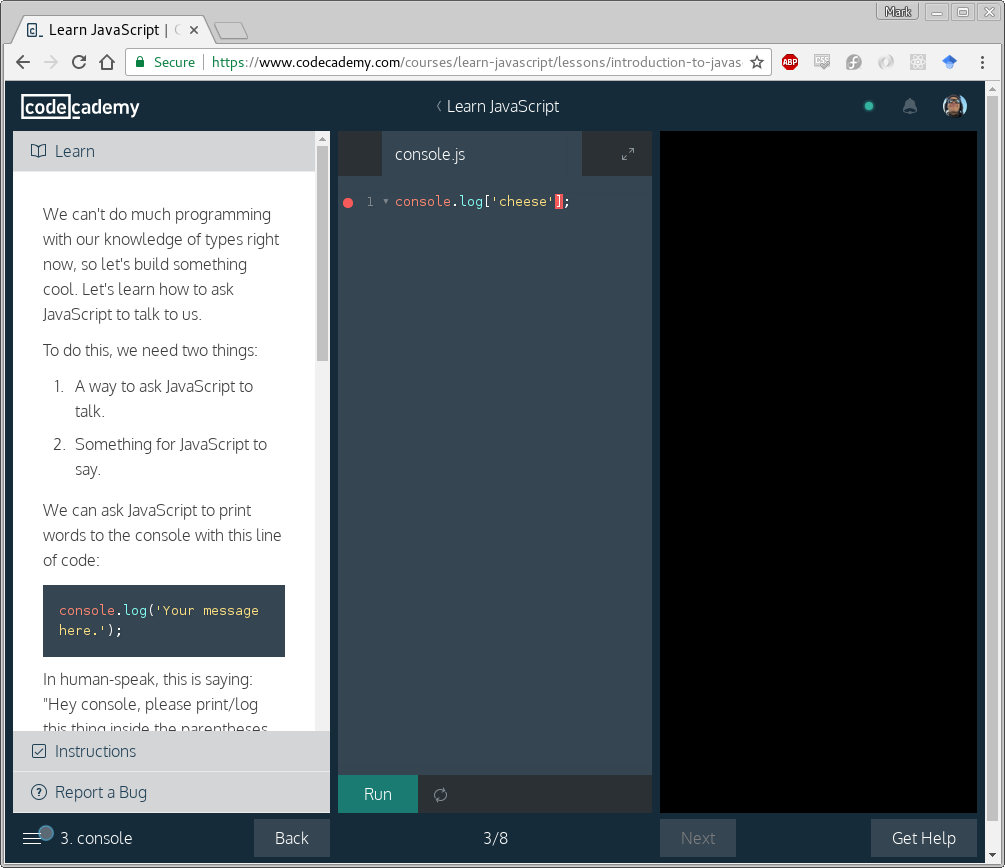
\includegraphics[width=\textwidth]{graphics/codecademy} % e.g. insert ./image for image.png in the working directory, adjust scale as necessary
\caption{Codecademy programming environment}
\label{fig:codecademy} % insert suitable label, this is used to refer to a fig from within the text as shown above
\end{figure}

The Codecademy programming environment designed for absolute novices is little more than a shallow wrapper around the JavaScript lexer, parser and interpreter. An experienced programmer who understands the notion of a method call would quickly realise their mistake and replace the square brackets with round ones. A novice would understand neither of the two error messages. The visual difference between the user's code and that given in the instructions is likely only a few pixels, but the computer understands it in a totally different way.

For a real-world programming language to provide meaningful error messages in this case, as well as all others that a novice could unwittingly encounter, would require an unacceptable level of complexity for a tool used by professionals. JavaScript is used for real business and the efficiency of its lexing and parsing stages is critical, as truly enormous sums of money have been invested in making it as fast and efficient as possible. Programmer-hours devoted to making JavaScript more suitable for novices are hours that cannot be spent on making the language more powerful for skilled users.

If there is no absolute requirement to use a real-world programming language to teach the essential complexity of programming, then why should it be done? An environment focussed on novices that uses only simple toy languages to explain the essential concepts would reduce the risk of an untutored learner making trivial mistakes that would prevent them progressing to more complex concepts that they would understand. As they become confident with the concepts, the essential complexity of real languages could be slowly introduced.

\section{Visual Programming for Novices}
A number of projects over several decades have created visualisation systems intended for novice programmers \cite{Sorva:2013:RGP:2543488.2490822}. Many of these have resulted in only short-term research prototypes focussed on one specific programming language, or even designed solely for visualising specific algorithms selected or created by an educator.

The recurring theme with these visualisations is that they are intended to help the programmer with the notional machine \cite{doi:10.2190/3LFX-9RRF-67T8-UVK9}: the extent of the computer's understanding as distinct from the programmer's. The novice programmer is able to watch the internal behaviour of this machine as it executes the code. The programmer is expected to learn to understand the limits of the machine in following each of the instructions literally. \cite{Sorva:2013:NMI:2483710.2483713}

A variety of studies in programming education have indicated that novice programmers ascribe human-like reasoning abilities to computers\cite{ragonis2005long}, or worse have little or no understanding of its behaviour and rely upon guesswork to complete assignments. Other problems relate to implicit or unexpected changes of state within the computer, such as updates to variable values. As the code is unchanging the relation of the text symbols in the code to their current values, and thus the actions of the computer in response to them, is hard for some novices to grasp. Beyond the novice stage, there can be a lack of understanding of the nature of higher-level concepts such as recursion or the difference between variable locations (e.g. static, heap or stack allocation) \cite{learnerMisconceptions}

Competent professional programmers have the use of powerful debugging tools at their disposal which can visualise the behaviour of their code and demonstrate these concepts, but these tools are designed by professionals for professionals. Teaching these tools alongside the art of programming itself simply adds to the burden; those who are able to quickly pick up the tools are likely also those who would pick up programming quickly, while those who require more assistance would require even more so.

A low-tech solution to the visualisation and understanding problem is to draw the whole state of the machine after each operation. These static visualisations can be presented to novices to demonstrate the changes caused by each, and to demonstrate the deterministic nature of computation. Questions can be asked of what the state should be after the next step of computation; comparing against the actual result should correct or reinforce the novice programmer's understanding \cite{1612204}. Clearly this is a tedious approach which does not scale with increasing program size and complexity. Given the graphical and processing capabilities available with commodity computing hardware, there should be no reason to slow down learning beyond what the user themselves requires.

The tedium of an enforced step-by-step manual calculation of computer state also has the serious problem of learner engagement. Few skills can be acquired without the learner actively wanting and able to participate. Static visualisations provide little scope for novel discoveries and experimentation, the likes of which would encourage a learner to stay focussed and wanting to continue. Allowing a novice to play around and see that some parts of their code are more significant than others provides the best opportunity to explain the underlying concepts - e.g. how changing one symbol can cause the program to loop forever.

A recurring theme of the programming visualisation systems to date is that they focus upon the visualisation of a real programming language. One reason for this is that many of these tools came about as an extension of the standard CS1 teaching programmes which already taught a specific language. If the course is to teach Pascal or Java, then it follows that tools created to help with that course would have novices use that language. Of the tools analysed by Sorva et al \cite{Sorva:2013:RGP:2543488.2490822}, only DISCOVER focuses on a pseudocode language written and displayed in an inherently beginning-friendly way. All others feature a standard programming text editor and some real language, often Java (being the CS1 language of choice for many institutions \cite{Hristova:2003:ICJ:792548.611956} as a demonstration of Object Oriented Programming). As outlined in the previous section, the use of a real-world programming language is inherently problematic for novices. While novices may be able to experiment with changing variable values or replacing certain symbols, any larger changes would likely result in an invalid program and a series of incomprehensible error messages. One unbalanced bracket can bring an experimenting novice to a grinding halt, causing frustration and hindering engagement with the learning environment.

The use of a real language in a standard programming text editor has also limited the scope for visualising the behaviour of the computer. All but a handful of the visualisation tools have a user interface consisting of a text entry box to one side or in one corner, and then the rest of the window filled with a variety of visualisations of the stack track and current variable values. Relations between the visualisation parts and the code itself are weak or non-existent, often consisting of little more than a selection of the current line of code being executed. The novice programmer is left to have to connect the visualisations to the code themselves, a task made more challenging by the abstract and convoluted nature of many of these visualisations. To make matters worse, effectively the entire computer state is visualised at once, meaning that the connections that should be made are less obvious than they could be. Highlighting only entire lines of code is problematic when there may be many operations on that single line. A simple assignment statement with a primary expression or single-level binary expression may be easy enough to follow within a line, but the same would not apply for the complex multi-level expression evaluations which are legal and common in real code.

A further problem with many of these visualisation tools is that they exist only for a single language, or possibly a set of languages implementing similar features. All but a couple exist only to visualise imperative alone or imperative plus object-oriented programming paradigms. These may be the most common paradigms but they are by no means the only ones in existence or worth teaching to novices. The vital part of programming education is not to each a specific language, but the underlying concepts of programming that apply equally to effectively all languages. Allowing only a limited range of languages and paradigms limits the teaching power of any tool, especially as comparing and contrasting between different approaches is as useful a teaching mechanism as teaching them in isolation. Building a visualisation tool around a single language or paradigm limits the imagination of how a computer can and should work, and how to best explain it to a novice. Even after a programmer has learned one language or paradigm, a visualisation tool may be extremely useful for them to learn another if it has very different underlying concepts and semantics. On a simple effort level, having multiple different projects for visualisation tools for different languages will result in wasted effort re-implementing the same common features over and over again, while denying the opportunity to simplify and abstract over these concepts for the benefit of both the tool creator and user.

The age of these tools has also had the effect of making them obsolete. Some of these tools were written for the original Macintosh or early Windows or DOS platforms, making them difficult or impossible to use today. Good tools have become obsolete, forcing newer educators and researchers to re-implement the wheel rather than advancing the field. While some of the more recent tools have been written in cross-platform languages and frameworks like Java and its GUI toolkits, some others have been written specifically for one platform in native code. As time goes on and the platforms for which they were written become obsolete, yet more tools will be effectively lost to the world.

In addition, there has been a massive shift of computing away from traditional full-featured platforms such as desktop computers and towards phones, tablets and the web as a platform. These platforms are actively designed to prevent arbitrary code execution due to security concerns, and have new and incompatible APIs that prevent even previously cross-platform code (such as Java applications) from running. While the underlying technology behind them has also enabled open computer education tools such as the Raspberry Pi to become widespread, any tool that cannot be used on the orders of magnitude more devices that can't create and run their own native programs is eventually doomed to failure. Emulation systems provide some possibility of these tools continuing to function well into the future on these new sandboxed platforms, but they cannot fix the fundamental shifts of how people interact with their computers. A desktop tool designed for a keyboard and mouse will not function optimally on a touchscreen device. If the tools have any dependency upon proprietary software, such as the Windows API, then future rights to distribute and understand the tool is also a legal grey area.

\section{Comparable projects and inspiration}

\subsection{Scratch}

Scratch was developed at the MIT Media Lab for use by children \cite{Resnick:2009:SP:1592761.1592779}. It provides a totally visual programming environment where program elements are represented as jigsaw-like blocks which can be connected together to create interactive programs. The range of capabilities of the language is geared around its target audience of young children, focussing on multimedia and the control of sprites on a canvas.

\begin{figure}[H]
\centering
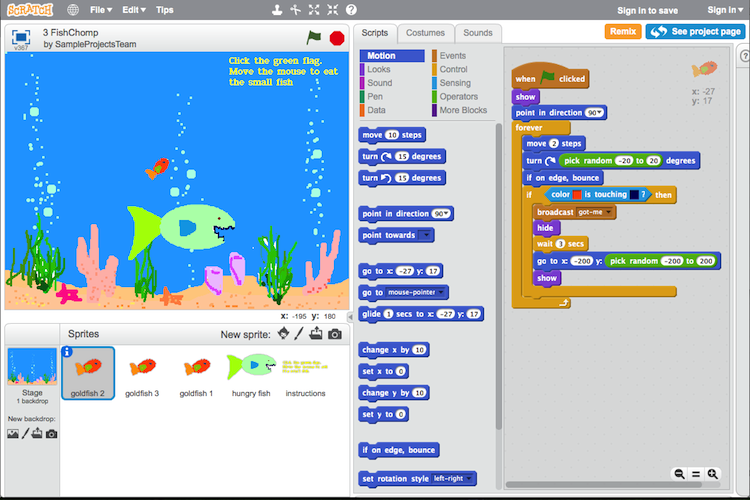
\includegraphics[scale=0.5]{graphics/scratch-editor} % e.g. insert ./image for image.png in the working directory, adjust scale as necessary
\caption{Scratch programming environment}
\label{fig:scratch} % insert suitable label, this is used to refer to a fig from within the text as shown above
\end{figure}

Scratch is a useful tool for its target audience but I feel that it is less than suited for many novice programmers, who may want a slightly more sophisticated and open-ended system. While Scratch may still be able to teach these people the basics of programming, its inherently simplistic and toy-like appearance may turn people away. It is quite possible that a novice programmer may be attempting to automate or speed up aspects of their own professional work. A novice programming tool that could include these use-cases therefore may be particularly useful.

\subsection{Lamdu}

Lamdu aims to create a "next-generation live programming environment that radically improves the programming experience" \cite{lamdu}. Lamdu programs can only be edited within the project's graphical code editor, which is implemented as a native application built on Haskell. The language is a purely functional language with similar syntax and semantics as Haskell, but designed specifically for visualisation within the graphical environment. This is the only language supported by the environment. The restriction to a single pure language, with no risk of adverse side-effects, allows the visualisations to include live evaluation of the program code. For example, the expression \verb+sum (1..1000)+ is immediately evaluated and its result (499500) displayed underneath.

\begin{figure}[H]
\centering
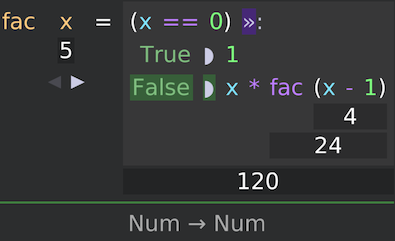
\includegraphics[scale=0.5]{graphics/lamdu} % e.g. insert ./image for image.png in the working directory, adjust scale as necessary
\caption{Example code within Lamdu programming environment}
\label{fig:scratch} % insert suitable label, this is used to refer to a fig from within the text as shown above
\end{figure}

While Lamdu includes other advanced functional language features of note, it is the visual presentation of the program which inspired me the most. I believe that this approach could be applied to any type of programming language, and that it could be implemented in a system that would be much more accessible than a native application with a complicated installation procedure.

\subsection{Learnable Programming by Brett Victor}

Brett Victor is a former UI designer for Apple Inc. Writing in a non-academic blog setting, he set out reasons why the way that we teach programming to novices is not fit for purpose \cite{BrettVictor}. He argues that the entire way in which we teach programming to novices is wrong, as we force them to use tools which withhold too much information from the programmer while allowing them to become confused about what their code should do. In his opinion, fixing this requires a considerable re-think of the entire programming environment, from the language to the development cycle. The design principles he outlines are framed as a series of questions:

Does the environment allow the learner to...
\begin{itemize}
\item read the vocabulary? -- Is meaning transparent? Is meaning explained in context, by showing and telling?
\item follow the flow? -- Is time visible and tangible? At all meaningful granularities?
see the state? -- Does the environment show the data? Show comparisons? Is hidden state eliminated?
\item create by reacting? -- Is something on screen as soon as possible? Is the parts bucket on the floor?
\item create by abstracting? -- Can the programmer start concrete, then generalize?
\end{itemize}
Does the language provide...
\begin{itemize}
\item identity and metaphor? -- Is the computer's world connected to the programmer's world?
\item decomposition? -- Can the programmer break down her thoughts into mind-sized pieces?
\item recomposition? -- Can the programmer put diverse pieces together?
\item readability? -- Is meaning transparent?
\end{itemize}

The particular idea which I found most interesting in his essay is that of controlling execution and time. Rather than having the code simply run as fast as the computer will allow, from initialisation through to termination, his idea is that users should be able to scrub back and forth in time and see the state of the program at any point. For example, a program that incrementally draws a flower on the canvas he describes could be slowed down, paused or rewound to show how the computer performs each and every step. Each petal or blade of grass must be drawn individually by the computer, but if the computer runs at full speed the user may not understand this fundamentally sequential nature of computer behaviour. To them, a function in their code which draws a square may be as static as a shape description in an SVG or other graphics file.

This control of time could be applied to any sort of basic computation, not just displaying graphics on a canvas, and I believe that it would assist novices greatly.